\documentclass[conference]{IEEEtran}

\usepackage[T1]{fontenc}
\usepackage[utf8]{inputenc}
\usepackage{times}
\usepackage{amsmath}
\usepackage{graphicx}
\usepackage{booktabs}
\usepackage{array}
\usepackage{multirow}
\usepackage{xcolor}
\usepackage{tikz}
\usepackage{url}
\usepackage[hidelinks]{hyperref}

\usetikzlibrary{arrows.meta,positioning,shapes.geometric}
\graphicspath{{figures/}}

\newcommand{\code}[1]{\texttt{\detokenize{#1}}}
\newcommand{\projecttitle}{Nutrition-Aware Indian Food Recognition Using YOLO and Conservative Class-to-Database Mapping}

\begin{document}

\title{\projecttitle}

\author{
\IEEEauthorblockN{Jaspreet Singh}
\IEEEauthorblockA{
Department of Computer Science and Engineering\\
National Institute of Technology Srinagar\\
Kashmir 190006, India\\
Email: [student email]
}
}

\maketitle

\begin{abstract}
Food recognition is useful only when visual predictions can be connected to nutrition information that users can understand and act on. This paper presents an end-to-end Indian food recognition system that combines YOLO-based object detection, a curated 72-class Indian food dataset, and a nutrition mapping layer derived primarily from the Indian Nutrient Database. The central engineering problem is not only detecting food objects, but also resolving inconsistent food labels, regional dish names, and incomplete nutrition database coverage without producing misleading macro estimates. Five YOLO-format food datasets were merged into a canonical dataset containing 48,693 exported image-label pairs. A visual verification procedure confirmed that all 72 classes have actual image samples and identified three sample-level annotation issues. The nutrition pipeline produces 1,010 food records in SQLite, including five verified supplemental rows for dishes absent from INDB, and creates 103 precomputed detector-to-database mappings, including legacy deployed-model labels. For the expanded dataset, all 72 classes are mapped to safe nutrition entries with source metadata. The implemented FastAPI and Next.js prototype demonstrates a practical workflow in which uploaded food images are processed by a YOLO detector, matched to nutrition records, and converted into calorie and macronutrient feedback. The results show that careful class normalization, conservative nutrition mapping, and transparent source tracking are necessary for making food recognition systems credible in regional dietary settings.
\end{abstract}

\begin{IEEEkeywords}
food recognition, object detection, YOLO, Indian food dataset, nutrition mapping, dietary recommendation, computer vision
\end{IEEEkeywords}

\section{Introduction}

Image-based food logging promises a lower-friction alternative to manual diet tracking. A user can photograph a meal and receive a list of detected food items, serving estimates, and nutrition values. In practice, however, the problem is more brittle than ordinary object detection. Food is deformable, frequently occluded, and often visually ambiguous. Indian food adds another layer of difficulty: dishes vary by region, share ingredients and colors, and are named inconsistently across datasets. A class such as \code{rice} may appear as \code{WhiteRice}, \code{satham}, or \code{boiled rice}; chutneys may be visible only as small side portions; and biryani variants can differ by ingredients rather than global shape.

The project described in this paper was built around a simple premise: a food recognition system should not stop at labels. A detected label must be mapped to a nutrition entry before it becomes useful. That mapping step is a source of real error. A fuzzy string match may return a food with a similar name but a different macro profile. For example, a detector class for \code{palak_paneer} should map to spinach paneer, not to a generic paneer preparation. Similarly, a class with no suitable INDB entry should use a verified supplemental row or remain unavailable rather than receive an arbitrary substitute.

This paper makes three contributions. First, it describes a dataset engineering pipeline that merges five YOLO-format Indian food datasets into a 72-class canonical dataset. Second, it presents a conservative class-to-database mapping strategy that prioritizes explicit semantic mappings and source-backed supplemental rows before fuzzy matching. Third, it reports a working full-stack prototype that links detection, nutrition lookup, macro calculation, and user-facing recommendations.

The work is best understood as an applied system paper. It does not claim a new detector architecture. Instead, it addresses the glue code, data cleaning, and mapping decisions needed to make an object detector useful in a nutrition-aware application. These decisions are often left implicit, but in this domain they determine whether the system returns helpful information or plausible-looking misinformation.

\section{Related Work}

Food computing has been studied as a broad field connecting image analysis, dietary assessment, recommendation, and human behavior \cite{min2019food}. Early food recognition systems such as FoodCam showed that smartphone-based food recognition could support real-time logging workflows \cite{kawano2014foodcam}. Im2Calories framed the problem as a mobile vision food diary and highlighted the difficulty of estimating food energy from images alone \cite{meyers2015im2calories}. These systems motivate the present work, but they also show why recognition must be connected to a reliable nutrition layer.

Object detection methods are well suited to meal images because a single image may contain multiple food items. Two-stage detectors such as Faster R-CNN achieve strong detection performance by separating proposal generation and classification \cite{ren2015fasterrcnn}. One-stage detectors such as YOLO instead formulate detection as a direct regression and classification problem, which makes them attractive for interactive applications \cite{redmon2016yolo}. Later YOLO variants improved multi-scale prediction and practical deployment \cite{redmon2018yolov3}. The implementation in this work uses Ultralytics YOLO tooling because it supports the YOLO annotation format used by the collected datasets and integrates cleanly with Python services \cite{ultralytics2024}.

Dataset quality remains a limiting factor. General object detection benchmarks such as COCO provide standardized annotations and category definitions \cite{lin2014coco}. Regional food datasets rarely have that level of consistency. The source data used in this project contained overlapping dishes, spelling variants, regional synonyms, and different class naming conventions. Nutrition data introduces a second schema mismatch: detector labels are short machine-learning classes, whereas nutrition databases store descriptive dish names with preparation details. The mapping layer in this work is therefore treated as part of the model pipeline rather than as a simple lookup table.

\section{System Overview}

Figure~\ref{fig:pipeline} summarizes the implemented workflow. Source datasets are normalized into a canonical YOLO dataset. A YOLO detector processes uploaded images and returns bounding boxes with class labels. The backend then resolves each class through a precomputed mapping table. When a safe mapping exists, nutrition values are returned from SQLite. When no safe mapping exists, the service reports the missing nutrition value instead of fabricating one.

\begin{figure}[t]
\centering
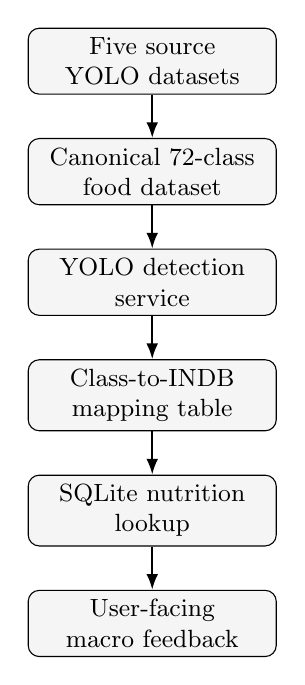
\begin{tikzpicture}[
    node distance=0.55cm,
    block/.style={draw, rounded corners, align=center, minimum width=3.15cm, minimum height=0.62cm, fill=gray!8, font=\small},
    arrow/.style={-{Latex[length=2mm]}, thick}
]
\node[block] (data) {Five source\\YOLO datasets};
\node[block, below=of data] (canon) {Canonical 72-class\\food dataset};
\node[block, below=of canon] (detect) {YOLO detection\\service};
\node[block, below=of detect] (map) {Class-to-INDB\\mapping table};
\node[block, below=of map] (nutrition) {SQLite nutrition\\lookup};
\node[block, below=of nutrition] (frontend) {User-facing\\macro feedback};
\draw[arrow] (data) -- (canon);
\draw[arrow] (canon) -- (detect);
\draw[arrow] (detect) -- (map);
\draw[arrow] (map) -- (nutrition);
\draw[arrow] (nutrition) -- (frontend);
\end{tikzpicture}
\caption{Pipeline from source datasets to nutrition-aware user feedback.}
\label{fig:pipeline}
\end{figure}

The backend is implemented with FastAPI, PyTorch, Ultralytics YOLO, Pillow, Pandas, OpenPyXL, SQLite, and AioSQLite. The frontend is implemented with Next.js, React, TypeScript, Tailwind CSS, and Lucide icons. The data layer contains the merged YOLO dataset, the INDB spreadsheet, the generated SQLite database, and detector weights. The deployed model metadata currently contains a smaller legacy class list, while the generated 72-class dataset is retained as the expanded training corpus.

\section{Dataset Construction}

The dataset pipeline was designed to produce stable class names before model training. Five YOLO-format source datasets were scanned for image and label folders. Labels were parsed in the standard YOLO form:
\begin{equation}
    y = (c, x, y, w, h),
\end{equation}
where $c$ is the class index and $(x,y,w,h)$ are normalized bounding-box coordinates. Each source class name was normalized into a canonical label through lowercasing, punctuation removal, synonym handling, and manual regional-name mappings.

Table~\ref{tab:dataset-summary} reports the generated split sizes. The final export contains 48,693 image-label pairs. Training data received augmentation, while validation and test splits were kept separate to avoid contaminating evaluation data.

\begin{table}[t]
\centering
\caption{Generated dataset split summary.}
\label{tab:dataset-summary}
\begin{tabular}{lrr}
\toprule
Split & Image-label pairs & Role\\
\midrule
Train & 36,852 & Training and augmentation\\
Validation & 5,922 & Model selection\\
Test & 5,919 & Held-out testing\\
\midrule
Total & 48,693 & Complete export\\
\bottomrule
\end{tabular}
\end{table}

The canonical dataset contains 72 food classes. It includes rice dishes, curries, breads, chutneys, snacks, desserts, beverages, and non-vegetarian dishes. Examples include \code{aloo_gobi}, \code{coconut_chutney}, \code{fish_curry}, \code{medu_vada}, \code{palak_paneer}, \code{sambar_satham}, and \code{veg_briyani}. The merge process also produced machine-readable artifacts such as \code{data.yaml}, build logs, and split count tables.

\subsection{Class Canonicalization}

The class normalization step was kept explicit because food-name variation is not a minor formatting problem. The same dish may appear with English spellings, regional names, camel-case names, or source-specific abbreviations. If these labels are not merged, the detector learns several partial classes for the same dish and the nutrition layer later receives inconsistent inputs.

Table~\ref{tab:canonicalization} gives examples of raw label variants and their canonical forms. The mapping dictionary was deliberately written in readable form so that a developer can audit each change. This is useful in food datasets because automatic string normalization alone cannot distinguish synonyms from visually related but distinct dishes.

\begin{table}[t]
\centering
\caption{Examples of source-label canonicalization.}
\label{tab:canonicalization}
\begin{tabular}{p{0.49\linewidth}p{0.34\linewidth}}
\toprule
Raw or source-side variants & Canonical class\\
\midrule
\code{AlooGobi}, \code{aloo gobhi}, \code{aloo_gobi} & \code{aloo_gobi}\\
\code{CoconutChutney}, \code{thengai chutney} & \code{coconut_chutney}\\
\code{WhiteRice}, \code{satham}, \code{rice} & \code{rice}\\
\code{medu vadai}, \code{medu vada} & \code{medu_vada}\\
\code{lemon satham}, \code{lemon rice} & \code{lemon_rice}\\
\bottomrule
\end{tabular}
\end{table}

The canonicalization pipeline also preserves multi-label images. If a source image contains more than one food object, each valid YOLO row is converted independently and written back to the exported label file. This avoids turning multi-dish meal images into single-label examples and keeps the object detection formulation intact.

\subsection{Visual Class Verification}

Class names were checked against actual images rather than accepted only from metadata. A verification script grouped exported images by canonical class suffix, sampled four images per class, parsed matching label files, and generated contact sheets. This process confirmed that all 72 classes have image samples and that the class list is aligned with the exported dataset.

\begin{figure}[t]
\centering

\includegraphics[width=\linewidth,height=0.38\textheight,keepaspectratio]{class_verification_page_01.jpg}
\caption{Example visual verification sheet generated from actual dataset images.}
\label{fig:verification}
\end{figure}

The review found three sample-level annotation issues: one file labeled as \code{jalebi} that does not visually resemble jalebi, one \code{kaara_chutney} bounding box placed on a vada rather than the chutney, and one \code{nandu_masala} label with an extremely thin bounding box. These issues are important, but they do not indicate a class-order failure. They point to local annotation cleanup work for a later dataset revision.

\section{Nutrition Mapping}

The nutrition layer imports the Indian Nutrient Database spreadsheet into SQLite \cite{indb_placeholder}. The final table contains 1,010 food records with calories, protein, carbohydrates, fat, and source metadata. Five rows are verified supplemental entries for dishes that are not present in the available INDB sheet. A second table, \code{yolo_mappings}, stores precomputed mappings from detector classes to nutrition database names.

The mapping algorithm follows a conservative order:
\begin{enumerate}
    \item normalize the detector class name;
    \item check an explicit manual mapping dictionary;
    \item check exact normalized database names;
    \item use a verified supplemental row when INDB has no safe row;
    \item use fuzzy matching only above a threshold;
    \item leave the class unavailable if no safe row exists.
\end{enumerate}

This order matters. Manual mappings catch semantic cases that string matching handles poorly. For example, \code{aloo_gobi} maps to \code{Potato cauliflower (Aloo gobhi)}, and \code{palak_paneer} maps to \code{Spinach paneer (Palak paneer)}. These are not merely similar strings; they are dish-level matches.

The mapping decision for a detector class $c$ can be written as:
\begin{equation}
M(c)=
\begin{cases}
M_{\mathrm{manual}}(c), & \text{if manually verified},\\
M_{\mathrm{exact}}(c), & \text{if normalized names match},\\
M_{\mathrm{sup}}(c), & \text{if a verified supplemental row exists},\\
M_{\mathrm{fuzzy}}(c), & \text{if score}(c) \geq 0.78,\\
\emptyset, & \text{otherwise}.
\end{cases}
\end{equation}
The final case is intentional. In a nutrition system, the cost of a wrong confident mapping can be higher than the cost of an absent mapping. A missing or supplemental mapping can be surfaced to the user with provenance; a wrong mapping silently corrupts calorie and macro feedback.

The final database contains 103 YOLO-to-database mappings. This number is larger than the 72 expanded classes because the table also includes legacy deployed-model labels for backward compatibility. For the expanded dataset alone, 72 of 72 classes are mapped, giving a class coverage of 100.00\%. The five classes absent from INDB are \code{bhakarwadi}, \code{ghevar}, \code{jalebi}, \code{khandvi}, and \code{nandu_masala}; they map to source-backed supplemental rows rather than weak fuzzy substitutes \cite{fatsecret_bhakarwadi_2026,clearcals_ghevar_2026,clearcals_jalebi_2026,clearcals_khandvi_2026,clearcals_nandu_kari_2026}.

\begin{table}[t]
\centering
\caption{Examples of detector-class to nutrition-database mappings.}
\label{tab:mapping-examples}
\begin{tabular}{p{0.28\linewidth}p{0.54\linewidth}r}
\toprule
Class & Database food name & Score\\
\midrule
\code{aloo_gobi} & Potato cauliflower (Aloo gobhi) & 1.00\\
\code{palak_paneer} & Spinach paneer (Palak paneer) & 1.00\\
\code{rice} & Boiled rice (Uble chawal) & 1.00\\
\code{chicken_biryani} & Chicken pulao & 0.80\\
\code{ven_pongal} & Plain khitchdi & 0.75\\
\bottomrule
\end{tabular}
\end{table}

The lower-confidence mappings in Table~\ref{tab:mapping-examples} are intentionally recorded with scores. They represent nearest safe substitutes rather than exact dish equality. This makes uncertainty visible to developers and avoids presenting approximate matches as ground truth.

\section{Application Prototype}

The runtime API accepts an image upload, runs YOLO inference, formats bounding boxes, and enriches each detection with nutrition values when available. The recommendation service uses a target calorie value, dietary goal, and optional health condition to produce macro guidance. The frontend displays detections, nutrition details, serving controls, and recommendations in a single workflow.

\begin{figure}[t]
\centering
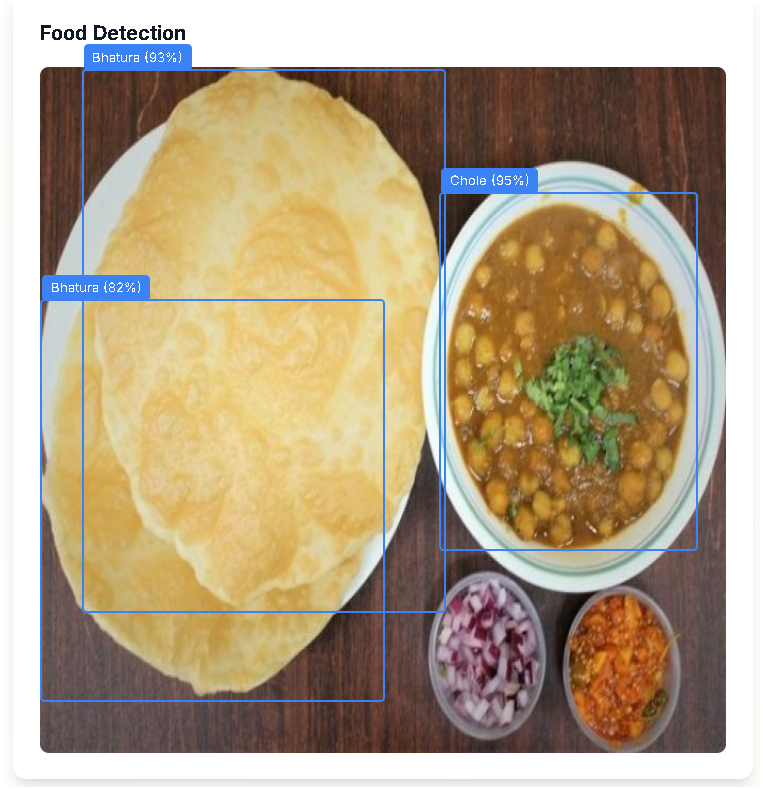
\includegraphics[width=\linewidth]{detection_overlay.png}
\caption{Prototype output showing detected food items with bounding boxes and nutrition-linked results.}
\label{fig:prototype}
\end{figure}

The design keeps detection and nutrition services separate. This separation avoids coupling model inference to database logic and makes it easier to replace either component. The mapping table also allows nutrition lookup to remain fast at runtime because expensive normalization and fuzzy matching are done during database build time rather than per request.

\section{Evaluation}

The evaluation focuses on dataset integrity, nutrition mapping coverage, and service-level behavior. Table~\ref{tab:evaluation} summarizes the main measured outcomes. The current paper does not report a full mAP table for the expanded 72-class model; that remains future work. Reporting only the measured system properties is preferable to presenting incomplete detector metrics.

\begin{table}[t]
\centering
\caption{System validation summary.}
\label{tab:evaluation}
\begin{tabular}{lr}
\toprule
Validation item & Result\\
\midrule
Canonical classes & 72\\
Exported image-label pairs & 48,693\\
Classes with visual samples & 72 / 72\\
Sample-level annotation issues found & 3\\
Nutrition food records & 1,010\\
Total YOLO-to-database mappings & 103\\
Expanded-class safe mappings & 72 / 72\\
Expanded-class mapping coverage & 100.00\%\\
\bottomrule
\end{tabular}
\end{table}

Several checks were also performed against the runtime lookup path. Representative classes such as \code{aloo_gobi}, \code{palak_paneer}, \code{rice}, \code{AlooGobi}, and \code{WhiteRice} returned the expected nutrition display names after the mapping revision. This confirmed that the updated pipeline supports both expanded dataset labels and legacy class names.

\subsection{Runtime Behavior Checks}

The system was tested at the service boundary because the user-facing behavior depends on more than the database contents. A successful response must carry the detector label, display name, confidence, bounding box, and nutrition values in a shape that the frontend can render. It must also fail gracefully when an image contains no recognized food or when a class lacks a nutrition mapping.

\begin{table}[t]
\centering
\caption{Runtime lookup behavior checked during validation.}
\label{tab:runtime-checks}
\begin{tabular}{p{0.33\linewidth}p{0.51\linewidth}}
\toprule
Input or condition & Expected behavior\\
\midrule
\code{aloo_gobi} & Return potato cauliflower nutrition row\\
\code{palak_paneer} & Return spinach paneer nutrition row\\
\code{WhiteRice} & Resolve legacy label to boiled rice\\
No detected food & Return no-food response without nutrition values\\
Unmapped class & Preserve detection and mark nutrition unavailable\\
\bottomrule
\end{tabular}
\end{table}

These checks are small, but they guard against regressions that ordinary model training metrics would miss. A detector can still produce a label while the application returns the wrong database row; conversely, the nutrition service can be correct while the frontend receives fields under unexpected names.

\section{Discussion}

The most important finding is that nutrition-aware food recognition depends on decisions outside the detector. Object detection gives a label and a location. A health-oriented application must decide what that label means nutritionally. When class names and database rows do not match exactly, the mapping layer becomes a source of domain error.

The conservative approach used here is useful because it avoids a common failure mode: returning a confident nutrition result for the wrong food. The five classes absent from INDB are handled through verified supplemental rows instead of weak substitutes. This is especially important for sweets, snacks, and seafood dishes where calories and macronutrient profiles vary widely by preparation.

The visual verification step also proved necessary. A metadata-only check would have confirmed class names and counts, but it would not have found the incorrect \code{jalebi} sample, misplaced \code{kaara_chutney} box, or thin \code{nandu_masala} annotation. The process is inexpensive and should be part of future dataset build runs.

Another practical observation is that backward compatibility matters during dataset expansion. The expanded dataset contains 72 classes, while the deployed model metadata still contains a smaller legacy class list. Rebuilding the mapping table only for the new dataset would break old model labels. The database builder therefore loads the expanded dataset classes first and then appends legacy labels. This keeps the application usable while the larger model is still being trained or evaluated.

\section{Threats to Validity}

The reported coverage numbers measure mapping and data integrity, not final dietary accuracy. A mapped class can still have portion-size uncertainty, and a database entry can differ from the exact recipe in the image. Indian dishes vary strongly by oil quantity, ingredient ratios, and regional preparation. For that reason, the system should be interpreted as a decision-support prototype rather than a clinical nutrition instrument.

The visual verification procedure is also sample based. Four examples per class are enough to find obvious class-order errors and some annotation problems, but they do not prove that every label in the dataset is correct. A future audit should combine contact-sheet review with automated checks for invalid boxes, empty crops, duplicate labels, and anomalous image-label pairs.

\section{Limitations and Future Work}

The current system has four main limitations. First, the expanded 72-class detector still needs a complete quantitative evaluation with mAP@50, mAP@50:95, per-class precision, per-class recall, confusion matrix, and latency. Second, portion estimation is not solved; nutrition values are returned per database serving basis and need user adjustment. Third, five classes rely on supplemental nutrition sources because the available INDB sheet is incomplete for those dishes. Fourth, the visual verification process found annotation noise that should be corrected before the next training cycle.

Future work should replace or cross-check supplemental nutrition rows with official Indian food composition entries, train and evaluate the expanded detector under fixed experimental settings, and add portion estimation using either depth cues, reference objects, or calibrated serving-size inputs. A review dashboard for class-wise annotation inspection would also make dataset maintenance easier.

\section{Conclusion}

This paper presented a practical nutrition-aware Indian food recognition system built around YOLO detection, dataset normalization, and conservative nutrition mapping. The work merged five YOLO-format datasets into a 72-class canonical dataset with 48,693 exported image-label pairs, verified the class list through actual image samples, produced 1,010 nutrition records, and mapped all 72 expanded classes to safe database entries. The resulting prototype demonstrates that regional food recognition requires more than a detector: it requires careful class naming, transparent database mapping, source provenance, and explicit handling of uncertainty. These engineering choices make the difference between a visually impressive demo and a system that can support credible dietary feedback.

\section*{Acknowledgment}

The implementation and dataset engineering artifacts used in this manuscript were developed as part of a final year project in the Department of Computer Science and Engineering, National Institute of Technology Srinagar.

\bibliographystyle{IEEEtran}
\bibliography{bibliography/references}

\end{document}
